\documentclass[usenames,dvipsnames]{beamer}
\usetheme{Antibes}
\usecolortheme{beaver}
\usepackage{lmodern}
\usepackage[italian]{babel} 
\usepackage[T1]{fontenc}
\usepackage[utf8]{inputenc}
\usepackage{subcaption}
\usepackage{amsmath}
\usepackage[customcolors]{hf-tikz}
\usepackage{empheq, mathtools}
\usepackage{xcolor}
\usepackage{tikz}
\usepackage{hyperref}
\usepackage{enumitem}
\setbeamertemplate{footline}[frame number]




\title{Bayesian approach to Extreme Value Theory}
\subtitle{How to study unusual weather events?}
\author{Davide Fabbrucci, Matteo Pierdomenico, Giacomo Randazzo}
\institute{Politecnico di Milano}
\date{07/01/2021}
%%%%%%%Cose utili
% \hspace{1.5cm}
% \vspace{1.5cm}
% \bigskip
% \fontsize{3mm}{4mm}

\begin{document}

\begin{frame}
\titlepage
\end{frame}
\section{Resuming}

\begin{frame}
\frametitle{A brief recap of our data}
\small

\vspace{10pt}
Data: $\{x_{s,t}\}_{s \in S,t \in T} $ where \\
$x_{s,t} =\textit{intensity of daily highest wind gust(km/h)} $, \\
$S:=\{\textit{5 different counties of Ireland}\}$,\\
$T:=\{\textit{30 years of daily measuraments, about 11'000 observations}\}$. 
\begin{figure}[h!]
 \centering
  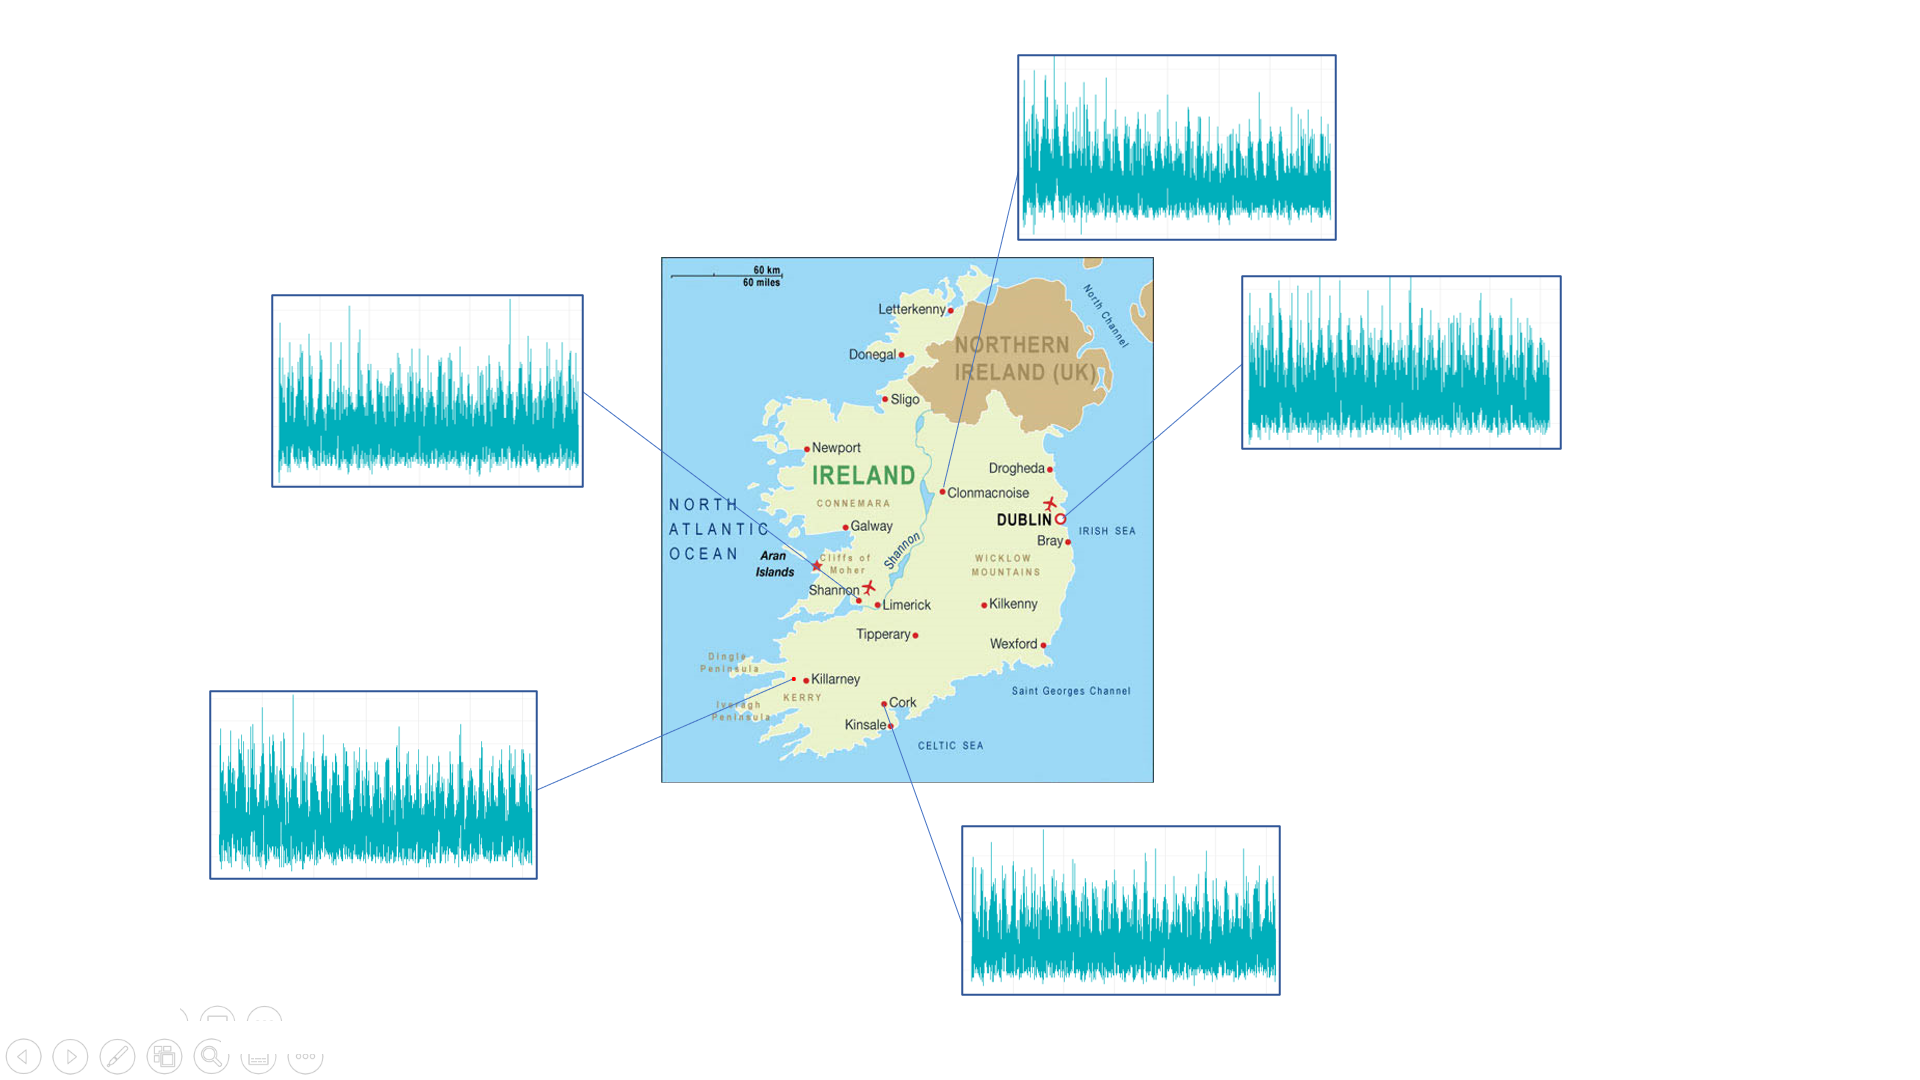
\includegraphics[width=0.9\textwidth]{ireland.png}
 \end{figure}

\end{frame}


\begin{frame}{Approaches to select extreme data from time series}
\small
    $\bullet$ \textit{Block Maxima approach}: \\
    $x_{\cdot,n}^{block-maxima}=\max\limits_{N\cdot (n-1) < t \leq  N \cdot n}{x_{\cdot,t}}$, where $N$ is the dimension of the block.  
       \begin{figure}[h!]
 \centering
  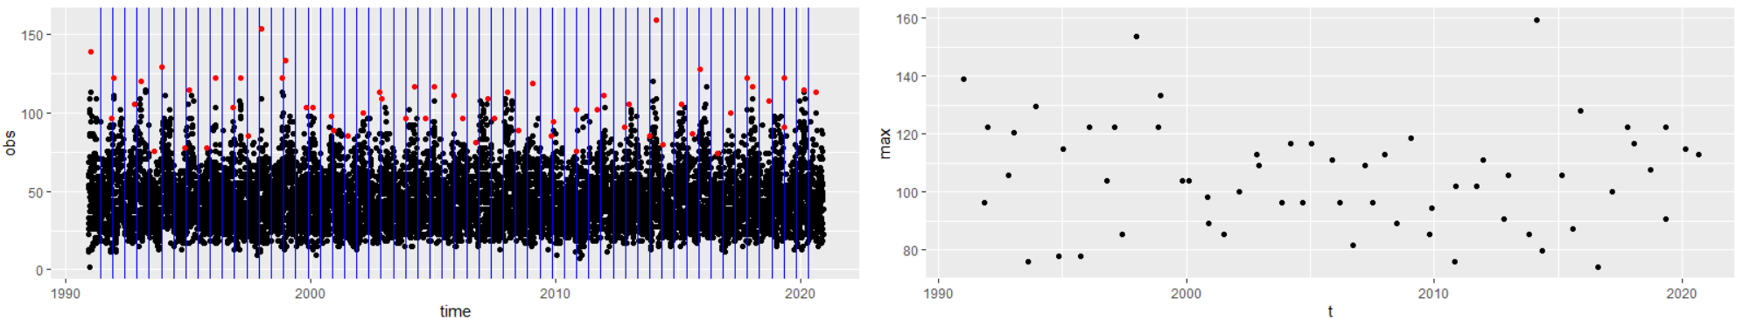
\includegraphics[width=1\textwidth]{BM_plot_1.png}
 \end{figure}
    
    $\bullet$ \textit{Peaks Over Threshold approach}:
    $x_{\cdot,t}^{POT}=x_{\cdot,t} \;\; s.t \;\; x_{\cdot,t} \geq threshold$
\begin{figure}[h!]
 \centering
  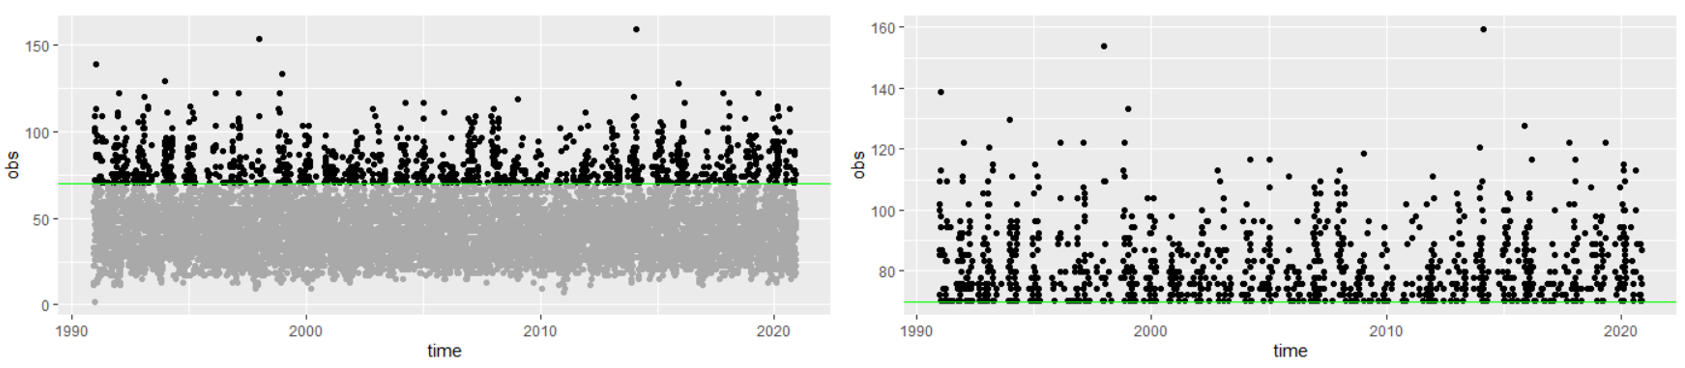
\includegraphics[width=1\textwidth]{POT_plot_1.png}
 \end{figure}
 
\end{frame}
\subsection{}

\section{Assumptions for first models}

\begin{frame}{Temporal dependence assumptions}
\small
 $\bullet$ Short-range dependence:\\
 The plot of the time series against the version at lag 1, for each site, shows correlation between successive observations, so we have to make some assumptions: 
    \begin{itemize}
    
        \item -for \textit{Block Maxima} approach:    %since data are maximum over blocks
        taking blocks sufficiently large removes short-range dependence for extremes;
        \\
        \vspace{4pt}
        
        \item -for \textit{P.O.T.} approach: clustering the nearby peaks and 
        select the max of each cluster removes the correletion between possible successive extremes.
        \\
    \end{itemize}
%our data are extremes of dependent process ( or equivalently extremes of stationary time series of observations)
$\bullet$ Long-range dependence:\\
We assumed long-range independence by using the \textit{Leadbetter's D condition}. %which guarantees that long-range dependence on observations $(x_{t}, x_{t+M}), M>>0$ is sufficiently weak to not to affect the asymptotics of an extreme value analysis.
\\
\end{frame}

\section{First models}

\begin{frame}
\frametitle{A first model: \textbf{Block Maxima approach} with STAN}
\footnotesize
Fixing $s \in S$:
\begin{equation*}
    x_{s,\cdot}^{block-maxima}|\mu,\sigma,\xi \sim \mathcal{GEV}(\mu,\sigma,\xi),
\end{equation*}   
\begin{equation*}
    \mu \sim \mathcal{N}\textit{(0, 10000)},
\end{equation*}
\begin{equation*}
    \sigma \sim \Gamma\textit{(0.001, 0.001)},
\end{equation*}
\begin{equation*}
    \xi \sim \mathcal{N}\textit{(0, 10)},
\end{equation*}

\vspace{12pt} 
where the CDF of the GEV distribution is 
\begin{equation*}
G(x)=exp \bigg\{-[ 1+\xi( \frac{x-\mu}{\sigma})^{\frac{1}{\xi} }]\bigg\},
\end{equation*}   
defined on the set $\{ x: 1 + \xi( \frac{x-\mu}{\sigma})>0\}$ with $\sigma > 0$. 
\end{frame}

\begin{frame}
\frametitle{Results for \textit{Clare county }}
\begin{figure}[h!]
 \centering
  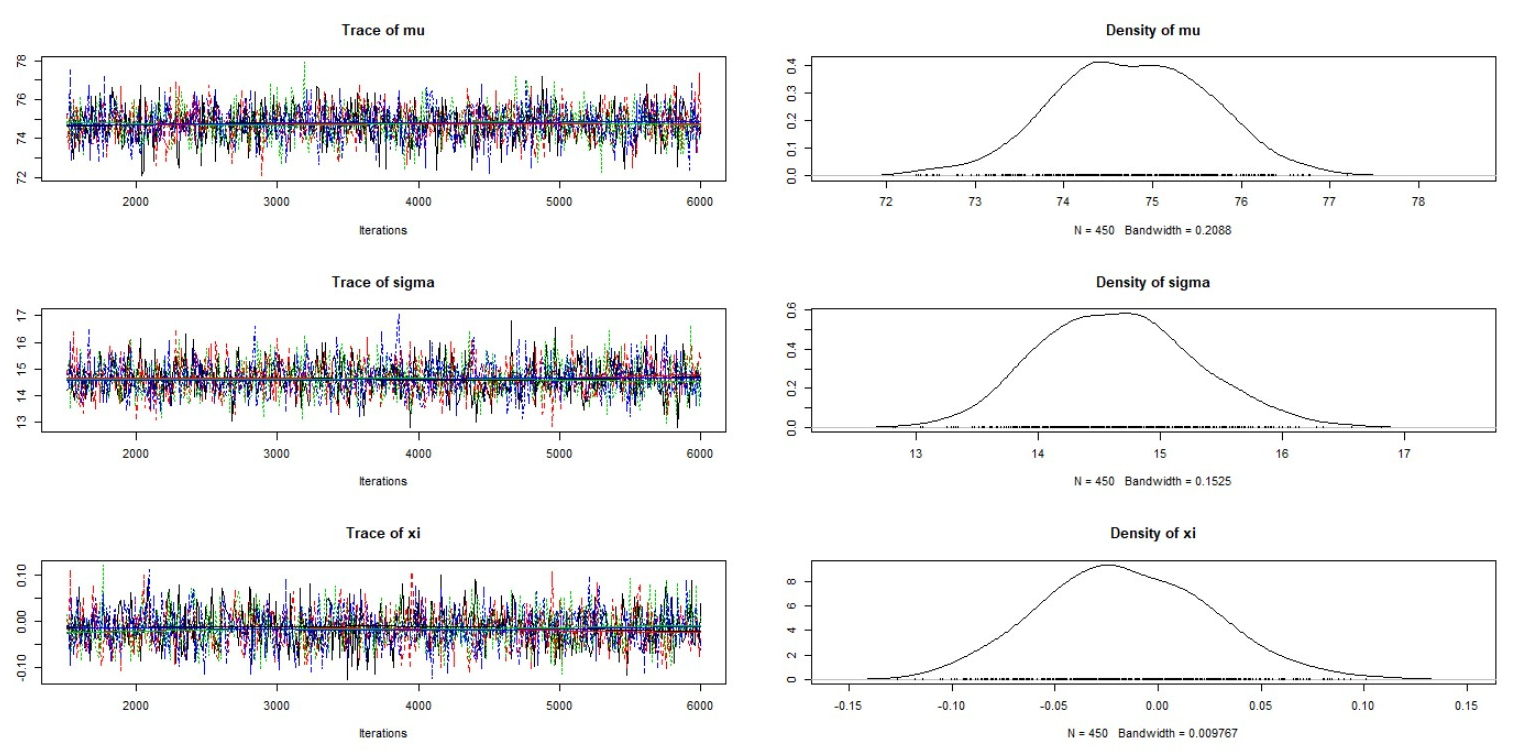
\includegraphics[width=1\textwidth]{coda_plots.png}
 \end{figure}
 
\end{frame}


\begin{frame}
\frametitle{Results for \textit{Clare county }}

\begin{center}
\begin{tabular}{ |c|c|c|c| } 
\hline
\textbf{Parameter}&\textbf{Mean}&\textbf{SD}\\ 
\hline

			\mu &74.77&0.88\\
\hline
			\sigma &14.65&0.64\\
\hline
			\xi &-0.02& 0.04\\
\hline
\end{tabular}
\end{center}


\begin{figure}
  \centering
  \begin{subfigure}[b]{0.4\textwidth}
    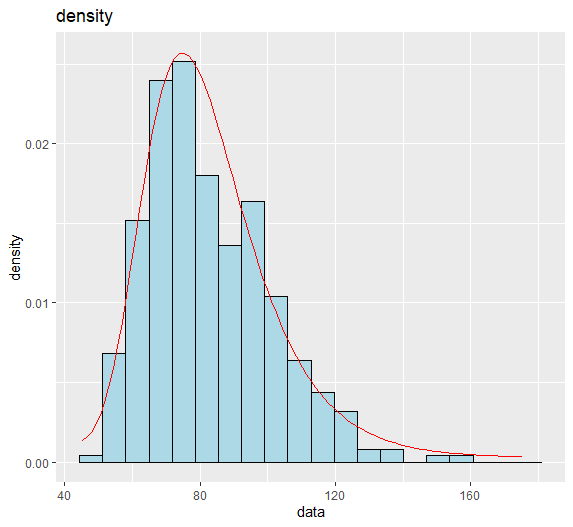
\includegraphics[width=\textwidth]{clare30density.png}
    \caption{Pointwise Predictive Density}
    \label{fig:sub1}
  \end{subfigure}
  \hfill
  \begin{subfigure}[b]{0.4\textwidth}
    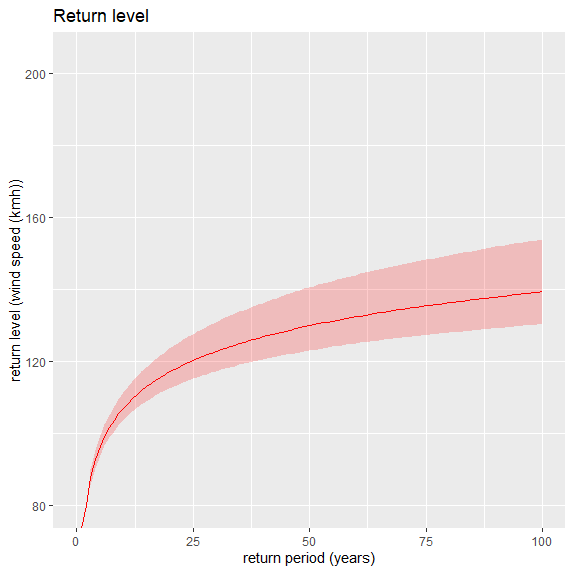
\includegraphics[width=\textwidth]{RetLev.png}
    \caption{Return Level}
    \label{fig:sub1}
  \end{subfigure}
\end{figure}
    
\end{frame}

\begin{frame}{Consideration about the priors}
\small
 \textcolor{red}Q: 
 \textcolor{black}Can we extract information from our data?\\
Fixing a location $s \in S$, we divided our set of daily observations $\{x_{s,t}\}_{t=1}^{T}$ in two parts: $\{x_{s,t}\}_{t=1}^{T^{*}}$ and $\{x_{s,t}\}_{t=T^{*}+1}^{T}$, $T^{*}\approx T/2$. \\
We then adopted the \textit{Block Maxima approach} model with non-informative priors for the first part of observations  $\{x_{s,t}\}_{t=1}^{T^{*}}$ in order to generate an MCMC sample of each parameter with which we gave informations to the priors of the \textit{Block Maxima approach} model for the second part of data $\{x_{s,t}\}_{t=T^{*}+1}^{T}$, i.e. : \\
\small
\begin{equation*}
    x_{s, \cdot}^{block-maxima}|\mu,\sigma,\xi \sim GEV(\mu,\sigma,\xi), 
\end{equation*}
\begin{equation*}
    \mu \sim \Gamma\textit{(3593.95, 48.47)},
\end{equation*}
\begin{equation*}
    \sigma \sim \Gamma\textit{(240.27, 16.78)},
\end{equation*}
\begin{equation*}
    \xi+\frac{1}{2} \sim \Gamma\textit{(68.68, 124.98)},
\end{equation*}

Results for \textit{Clare county}: $WAIC_{non-informative}= 1561.9$  $WAIC_{informative}= 1596.9$
    
\end{frame}


\begin{frame}
\frametitle{A first model: \textbf{Peaks over thresholds approach} with JAGS}
\small
Fixing $s \in S$, $u_1$ lower bound for the threshold (also used for declustering) and $u_2$ upper bound for the threshold:
\begin{equation*}
    x_{s,\cdot}^{POT, u_1}|\sigma,u,\xi \sim \begin{cases}
    \frac{1}{2}\frac{1}{(u - u_1)}       & \quad \text{if } u_1 \leq x < u\\
    \frac{1}{2}h(x | \sigma, u, \xi)  & \quad \text{if } x \geq u
  \end{cases},
\end{equation*}   
\begin{equation*}
    \sigma \sim \Gamma\textit{(0.001, 0.001)},
\end{equation*}
\begin{equation*}
    u \sim \mathcal{N}\textit{($u^{guess}_s$, $\sigma^2_{u^{guess}_s}$)}, \quad u \in (u_1, u_2),
\end{equation*}
\begin{equation*}
    \xi \sim \mathcal{N}\textit{(0, 10)}, \quad \xi \in \left( -\dfrac{\sigma}{x_{max} - u}, + \infty \right),
\end{equation*}

\vspace{10pt} 
where $h(x|\sigma, u, \xi)$ is the PDF of the GPD distribution.

\end{frame}









\begin{frame}
\frametitle{Results for \textit{Clare county}}
\begin{figure}[h!]
    \centering
    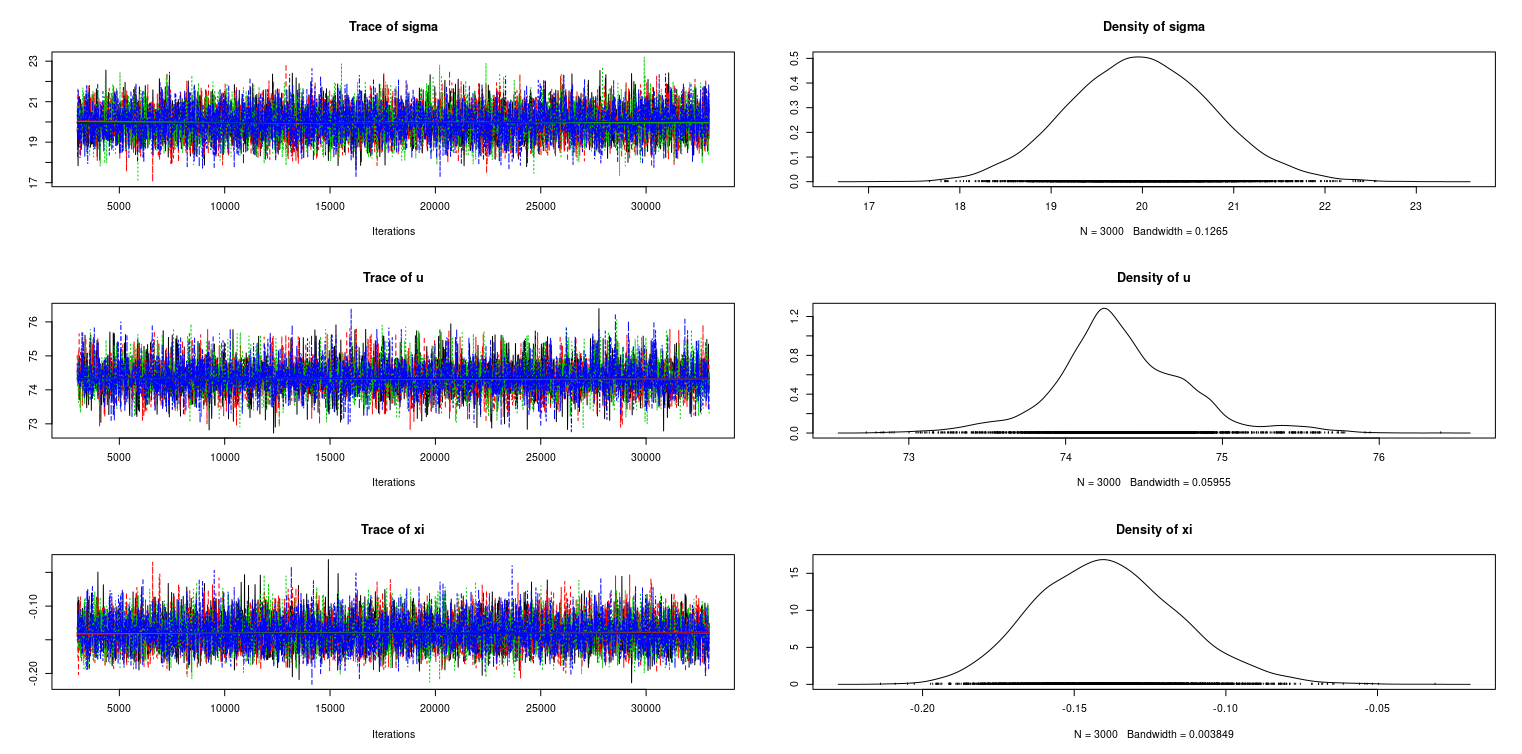
\includegraphics[width=1\textwidth]{coda_plot_GPD.png}
\end{figure}
     
\end{frame}










\begin{frame}
\frametitle{Results for \textit{Clare county}}
   \begin{center}
        \begin{tabular}{ |c|c|c|c| } 
            \hline
            \textbf{Parameter}&\textbf{Mean}&\textbf{SD}\\ 
            \hline

			u &70.70&0.56\\
            \hline
			\sigma &18.47&1.22\\
            \hline
			\xi &-0.10&0.04\\
\hline
\end{tabular}
\end{center}
\begin{figure}
  \centering
  \begin{subfigure}[b]{0.4\textwidth}
    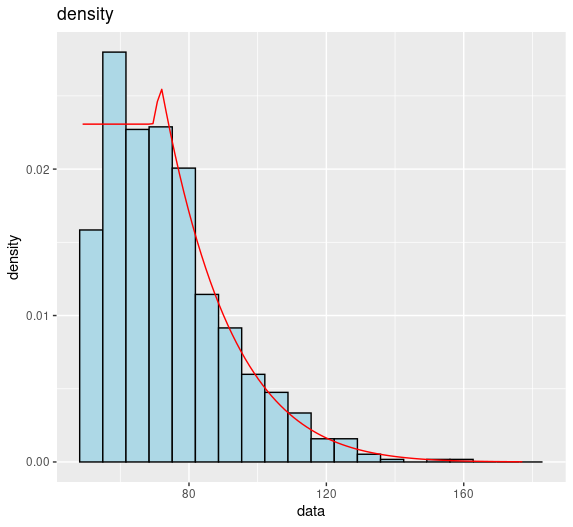
\includegraphics[width=\textwidth]{clare30DensityGPD.png}
    \caption{Pointwise Predictive Density}
    \label{fig:sub1}
  \end{subfigure}
  \hfill
  \begin{subfigure}[b]{0.4\textwidth}
    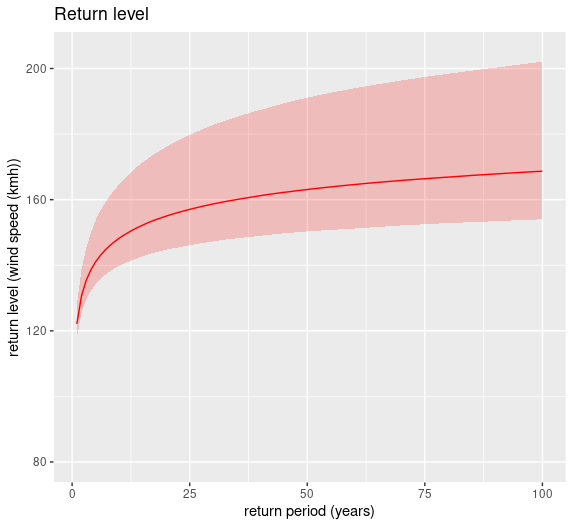
\includegraphics[width=\textwidth]{retLevGPD.png}
    \caption{Return Level}
    \label{fig:sub1}
  \end{subfigure}
\end{figure}
     
\end{frame}


\section{Hierarchical model}
\begin{frame}{A random effect model for spatiotemporal data}
\small
\textbf{Problem:} We have observations in five different sites and, in each site, extreme wind gust can suffer from seasonal variation. How can we model this variability in our analysis of extremes? 
\\
\vspace{8pt}
\textbf{Solution:} Fitting a site-seasonal varying \textit{GPD}! 
\\
\vspace{8pt}
\textbf{Idea}: We partition the annual cycle in 12 "seasons" (months actually) for each site, %reflects better the seasonal changing
thus our model will yeld parameters pairs
\begin{equation*}
(u_{s,m},\sigma_{s,m},\xi_{s,m}), \hspace{20pt} s=1,...,5 \;\;\;  \;\;\; m=1,...,12
\end{equation*}
\frametitle{}
where s and m are indeces for site and season respectively.

\end{frame}

\begin{frame}
\frametitle{Hierarchical Random effects model}
\small
$\bullet$ \textbf{Assumptions}:
\begin{itemize}
    \item -the GPD is valid for exceedances over a high threshold for
each month at each site,
    \item -extremes between sites and between months are independent,
%Spatial dependence in weather at our sites should not translate to strong correlations between extremes across sites
    \item -there is no interaction between monthly and site effects, 
    \item -both spatial effects and monthly effects are exchangeable.
\end{itemize}
\\
\vspace{10pt}
So, the first layer of our model is:
\begin{equation*}
    x_{(s,m),\cdot}^{POT}|u_{s,m},\sigma_{s,m},\xi_{s,m} \sim \mathcal{GPD}(u_{s,m},\sigma_{s,m},\xi_{s,m}), \;\;\; for \;\;\; m=1,...,12 \;\;\; \\ \hspace{220pt} \;\;\;\;\; $s=1,...,5$.
\end{equation*}   

\end{frame}
\section{Hierarchical model}

\begin{frame}
\frametitle{Hierarchical Random effects model}
\small
Building the random effects:
\begin{equation*}
    log(\sigma_{s,m})= \epsilon_{\sigma}^{(s)}  + \gamma_{\sigma}^{(m)}
\end{equation*}
\begin{equation*}
    log(\xi_{s,m})= \epsilon_{\xi}^{(s)}  + \gamma_{\xi}^{(m)}
\end{equation*}
where we take $log(\sigma_{s,m})$ to retain the positivity of the scale parameter $\sigma_{s,m}$.\\

All random effects are normally and independently distributed:
\begin{equation*}
    \epsilon_{\cdot}^{(s)} \sim \mathcal{N}\textit{$(a_{\cdot}, 1/\xi_{\cdot})$}, \;\;\; for \;\;\; s=1,...,5 \;\;\; \; the \;  site\;  effect,
\end{equation*}
\begin{equation*}
    \gamma_{\cdot}^{(m)} \sim \mathcal{N}\textit{$(0, 1/\tau_{\cdot})$}, \;\;\; for \;\;\; m=1,...,12 \;\;\; \; the \;  monthly\;  effect.
\end{equation*}
The final layer is then: %we adopt conjugacy to simplify the computations
\begin{equation*}
    a_{\cdot} \sim \mathcal{N}\textit{(0, 1000000)}, \;\;\xi_{\cdot}\sim \Gamma\textit{(0.01, 0.01)}, \;\; \tau_{\cdot}\sim \Gamma\textit{(0.01, 0.01)}.
%highly non-informative priors
\end{equation*}
\end{frame}
\section{conclusions}
\begin{frame}
\frametitle{Objectives}
\\

Ultimating the implementation and the analysis of the Hierarchical random effect model.\\
\vspace{8pt}
\textbf{Modelling temporal dependence}: as seen before, in our data there is a serial correlation between successive observation in the \textit{POT} approach %so between consecutive extremes 
\\
\begin{itemize}
    \item -A simple way to handle it is by means \textbf{declusterization}.
    \item -A more difficult way, but very interesting, is to \textbf{explicitly model} it by means of a first-order Markov model. % i.e. in the likelihood for the parameters, there will be a contribution by a joint distribution of consecutive observations,typically a bivariate logistic extreme value distribution 
    
    
\end{itemize}


\end{frame}



%%%%%%%%%%%%%%%%%%%%
\section{Bibliography}
\begin{frame}
\frametitle{References}
\begin{thebibliography}{2}
\tiny
\bibitem{EVT:1}
L.Fawcett,D. Walshaw.
\emph{Modelling Environmental Extremes}
Short Course for the 19th Annual Conference of The International Environmetrics Society, The University of British Columbia kanagan, Kelowna, Canada (2008)
\bibitem{EVT:2}
Jacob M., Neves C., Vukadinović Greetham D. (2020) 
\emph{Extreme Value Theory. In: Forecasting and Assessing Risk of Individual Electricity Peaks}
Mathematics of Planet Earth. Springer, Cham. 
\bibitem{EVT:3}
Behrens, C.N.; Lopes, H.F. & Gamerman, D. (2004). 
\emph{Bayesian analysis of extreme
events with threshold estimation}
Statist. Mod., 4, 227–244.
\bibitem{EVT:4}
N.A.M. Amina, M.B. Adam, A.Z. Aris
\emph{Bayesian Extreme for modeling high PM10 concentration in Johor }
Procedia Environmental Sciences 30 ( 2015 ) 309 – 314 
\bibitem{EVT:5}
Fawcett, L. and Walshaw, D.,
\emph{ A hierarchical model for extreme wind speeds.}
Journal of the Royal Statistical Society: Series C (Applied Statistics), 55: 631-646 (2006). 
\bibitem{EVT:6}
Behrens CN, Lopes HF, Gamerman D.
\emph{ Bayesian analysis of extreme events with threshold estimation.}
Statistical Modelling. 2004;4(3):227-244.
\bibitem{EVT:7}
Scarrott, Carl, and Anna MacDonald. 
\emph{Scarrott, Carl, and Anna MacDonald. A review of extreme value threshold es-timation and uncertainty quantification.}
REVSTAT–Statistical Journal 10.1 (2012): 33-60.
\end{thebibliography}
\end{frame}

\part{}
\begin{frame}[noframenumbering]
\frametitle{Leadbetter’s $D(u_{n})$ condition}
\scriptsize
Leadbetter’s $D(u_{n})$ condition ensures that long–range dependence is sufficiently weak so that it does not affect the asymptotics
of an extreme value analysis. This condition is stated more formally in this way:
\begin{definition}
A stationary series $x_{1}, x_{2}, ...$ is said to satisfy the $D(u_{n}$ condition if, for all $i_{1}<...< i_{p}<j_{1}<...<j_{q}$ with $j_{1}-i_{p}>l$, 
\begin{equation*}
    \Big|Pr\Big\{ x_{i_{1}}\leq u_{n},...,x_{i_{p}}\leq u_{n},x_{j_{1}}\leq u_{n},...,x_{j_{q}}\leq u_{n}\Big\}-
    \\
    \hspace{70pt} Pr\Big\{ x_{i_{1}}\leq u_{n},...,x_{i_{p}}\leq u_{n}\Big\}Pr\Big\{x_{j_{1}}\leq u_{n},...,x_{j_{q}}\leq u_{n}\Big\}\Big|\leq \alpha(n,l),
\end{equation*} \\
\\


where $\alpha(n,l) \rightarrow 0$ for some sequence $l_{n}$ s.t. $l_{n}/n \rightarrow 0$ as $n \rightarrow \infty$.
\end{definition}
$D(u_{n})$ condition holds only for a specific sequence of thresholds $u_{n}$ that increases with n. For such a sequence, the $D(u_{n})$ condition ensures that, for sets of variables that are far enough apart, the difference in probabilities in the definition is sufficiently close to zero to have no effect on the limit laws for extremes.
\end{frame}

\end{document}
